\section{Transaction Contracts}
\label{sec:txns}

While contracts on individual operations offer the programmer object-level
declarative reasoning, real-world scenarios often involve operations that span
multiple objects. In order to address this problem, several recent
systems~\cite{Walter,Burckhardt2012,BailisHAT} have proposed eventually
consistent transactions in order to compose operations on multiple objects.
However, given that classical transaction models such as serializability and
snapshot isolation require inter-replica coordination, these systems espouse
\emph{coordination-free transactions} that remain available under network
partitions, but only provide weaker isolation guarantees. Coordination-free
transactions have intricate consistency semantics and widely varying runtime
overheads. As with operation-level consistency, the onus is on the programmer
to pick the correct transaction kind. This choice is further complicated by
the consistency semantics of individual operations.

\subsection{Syntax and Semantics Extensions}
\label{sec:syn_sem_ext}

\name automates the choice of assigning the correct and most efficient
transaction isolation level. Similar to contracts on individual operations, the
programmer associates contracts with transactions, declaratively expressing 
consistency specifications. We extend the contract language with a new term
under quantifier-free propositions - ${\small \txnZ}~S_1~S_2$, where $S_1$ and
$S_2$ are sets of effects, and introduce a new primitive equivalence relation
$\small \sametxnZ$ that holds for effects from the same transaction. $\small
\txn{a,b}{c,d}$ is just syntactic sugar for $\small \sametxn{a}{b} ~\wedge~
\sametxn{c}{d} ~\wedge~ \neg\sametxn{a}{c}$, where $a$ and $b$ considered to
belong to the \emph{current} transaction.

We assume that operations not part of any transaction belong to their own
unique transaction. While transactions may have varying isolation guarantees,
we make the standard assumption that all transactions provide atomicity. Hence,
we include the following axiom in $\Delta$:

\begin{cmathpar}
\forall a,b,c.~\txn{a}{b,c} ~\wedge~ \sameobj{b}{c} ~\wedge~ \vis{b}{a}
\Rightarrow \vis{c}{a}
\end{cmathpar}

\noindent The semantics of this contract is illustrated in
Figure~\ref{fig:txn_atomicity}.

\subsection{Transactional Bank Account}

In order to illustrate the utility of declarative reasoning for transactions,
consider an extension of our running example to use two accounts (objects) --
current ($c$) and savings ($s$). Each account provides operations
\rcf{withdraw}, \rcf{deposit} and \rcf{getBalance}, with the same contracts as
defined previously. We consider two transactions -- \cf{save(amt)}, which
transfers \cf{amt} from current to savings, and \cf{totalBalance}, which
returns the sum of the balances of individual accounts. Our goal is to ensure
that \cf{totalBalance} returns the result obtained from a consistent snapshot
of the object states. The \name code for these transactions is given below:

\noindent \begin{minipage}[t]{0.53\columnwidth}
\begin{codehaskell}
save amt =
  x <- dollar(classify $\cv_{sv}$)
  atomically x dollar do
    b <- withdraw c amt
    when b dollar deposit s amt
\end{codehaskell}
\end{minipage}
\begin{minipage}[t]{0.47\columnwidth}
\begin{codehaskell}
totalBalance =
  x <- dollar(classify $\cv_{tb}$)
  atomically x dollar do
    b1 <- getBalance c
    b2 <- getBalance s
    return b1 + b2
\end{codehaskell}
\end{minipage}

$\cv_{sv}$ and $\cv_{tb}$ are the contracts on the corresponding
transactions. The function \cf{classify} assigns the contracts
\emph{statically} to one of the transaction isolation levels offered by the
store; \cf{\$()} is meta-programming syntax for splicing the result into the
program. The \cf{atomically} construct invokes the enclosing operations at the
given isolation level $x$, ensuring that the effects of the operations are made
visible atomically.

While making both transactions serializable would ensure correctness,
distributed stores rarely offer serializable transactions given their
availability requirements and implications for
scalability~\cite{BailisHAT}. Fortunately, these transactions can be
satisfied with much weaker isolation guarantees. However, despite the atomicity
offered by the transaction, anomalies are still possible. For example, the
two \rcf{getBalance} operations in a \cf{totalBalance} transaction might be
served by different replicas with a distinct set of committed \cf{save}
transactions. If the first(second) \rcf{getBalance} operation witnesses a
\cf{save} transaction that is not witnessed by the second(first)
\rcf{getBalance} operation, then the balance returned will be less(greater)
than the actual balance. It is not immediately apparent how to choose the weakest
isolation guarantee that would be sufficient to prevent the anomaly.

Instead, \name requires the programmer to simply state the consistency
requirement as a contract. Since we would like both the \rcf{getBalance}
operations to witness the same set of \cf{save} transactions, we define the
constraint on the \cf{totalBalance} transaction $\psi_{tb}$ as:

\begin{cmathpar}
\begin{array}{l}
\cv_{tb} = \forall a:\rcf{getBalance}, b:\rcf{getBalance}, \\
\qquad (c:\rcf{withdraw} \vee \rcf{deposit}), (d:\rcf{withdraw} \vee \rcf{deposit}). \\
\qquad \txn{a,b}{c,d} ~\wedge~ \vis{c}{a} ~\wedge~ \sameobj{d}{b} \Rightarrow \vis{d}{b}
\end{array}
\end{cmathpar}

\noindent The key idea in the above definition is that the $\small \txnZ$ primitive
allows us to relate operations on different objects.

The \cf{save} transaction only needs to ensure that the two writes it performs
are made visible atomically. Since this is ensured by combining them in a
transaction, \cf{save} does not require any additional constraints, and
$\psi_{sv}$ is simply $\small \true$.

\subsection{Coordination-free Transactions}

\begin{figure}
\centering
\subfigure[Atomicity]{
  \label{fig:txn_atomicity}
  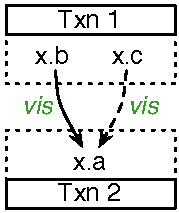
\includegraphics[width=0.25\columnwidth]{Figures/TxnAtomic}
}
\hfill
\subfigure[Monotonic Atomic View]{
  \label{fig:txn_mav}
  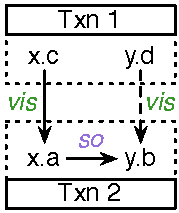
\includegraphics[width=0.25\columnwidth] {Figures/TxnMAV}
}
\hfill
\subfigure[Repeatable Read]{
  \label{fig:txn_rr}
  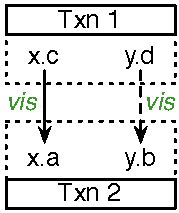
\includegraphics[width=0.25\columnwidth]{Figures/TxnRR}
}
\caption{Semantics of transaction contracts. $x$ and $y$ are distinct objects.
The dotted line represents the visibility requested by the contracts.}
\label{fig:transaction}
\end{figure}

In order to illustrate the utility of transaction contract classification, we
identify three well-understood coordination-free transaction semantics -- Read
Committed (RC)~\cite{Berenson95}, Monotonic Atomic View (MAV)~\cite{BailisHAT}
and Repeatable Read (RR)~\cite{Berenson95}, and illustrate the classification
strategy. Our technique can indeed be applied to a different isolation-level
lattice.

A transaction with ANSI RC semantics only witnesses committed operations. Let
us assume that a replica will buffer transactional updates until all the
updates from the same transaction are available at that replica. Once all the
updates from a transaction are available, the buffered updates are made visible
to subsequent client requests. This ensures atomicity of transactions.
Importantly, RC does not entail any other guarantees. As a result, a store
implementing RC does not require inter-replica coordination. We can express RC
as follows:

\begin{cmathpar}
\begin{array}{l}
\rcc = \forall a,b,c.~\txn{a}{b,c} \wedge \sameobj{b}{c} \\
\qquad \qquad \qquad \wedge~ \vis{b}{a} \Rightarrow \vis{c}{a}
\end{array}
\end{cmathpar}

\noindent Notice that the above definition is the same as the atomicity
guarantee of transaction described in \S~\ref{sec:syn_sem_ext}. The \cf{save}
operation is an example of an RC transaction.

MAV semantics ensures that if some operation in a transaction $T_1$ witnesses
the effects of another transaction $T_2$, then subsequent operations in $T_1$
will also witness the effects of $T_2$. MAV semantics is useful for maintaining
the integrity of foreign key constraints, materialized views and secondary
updates~\cite{BailisHAT}. In order to implement MAV, a store only needs to keep
track of the set of transactions $S_t$ witnessed by the running transaction,
and before performing an operation at some replica, ensure that the replica
includes all the transactions in $S_t$. Hence, MAV is coordination-free. MAV
semantics is captured with the following contract:

\begin{cmathpar}
\begin{array}{l}
\mavc = \forall a,b,c,d.~\txn{a,b}{c,d} ~\wedge~ \so{a}{b} ~\wedge~ \vis{c}{a} \\
\qquad\qquad\qquad\qquad ~\wedge~ \sameobj{d}{b} \Rightarrow \vis{d}{b}
\end{array}
\end{cmathpar}

\noindent whose semantics is illustrated in the Figure~\ref{fig:txn_mav}.

ANSI RR semantics requires that the transaction witness a snapshot of the data
store state. Importantly, this snapshot can be obtained from any replica, and
hence RR is also coordination-free. An example for such a transaction is the
\cf{totalBalance} transaction. The semantics of RR is captured by the following
contract:

\begin{cmathpar}
\begin{array}{l}
\rrc = \forall a,b,c,d.~\txn{a,b}{c,d} ~\wedge~ \vis{c}{a} \\
\qquad\qquad\qquad\quad ~\wedge~ \sameobj{d}{b} \Rightarrow \vis{d}{b}
\end{array}
\end{cmathpar}

\noindent whose semantics is illustrated in the Figure~\ref{fig:txn_rr}.

\subsection{Classification}

Similar to operation-level contracts, with respect to $\le$ relation, the
coordination-free transaction semantics described here form a total order:
$\rcc \le \mavc \le \rrc$. The transaction classification is also similar to
the operation-level contract classification presented in
Figure~\ref{sem:classify}; given a contract $\psi$ on a transaction, we start
from the weakest transaction contract $\rcc$, and progressively compare its
strength to the known transaction contracts until we find a isolation level
under which $\psi$ can be safely discharged. Otherwise, we report a type error.
